% !TEX root = main.tex
\begin{figure}[htbp]
\centering
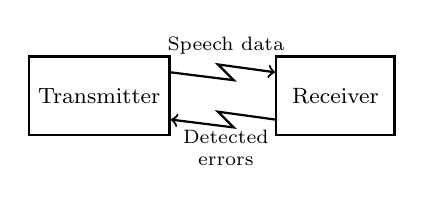
\begin{tikzpicture}[                
                    box/.style={
            		draw,
			thick,
            		text centered,
            		minimum width=1.5cm,
            		minimum height=1cm,
			font=\footnotesize,
			align=center,
			anchor=center,
            	} ]
	

\draw 
(0,0) node[box] (trans) {Transmitter}
(3,0) node[box] (rec) {Receiver}
(rec.west) ++(0,0.3) coordinate[](data_in) {}
(trans.east) ++(0,0.3) coordinate[](data_out) {}
(rec.west) ++(0,-0.3) coordinate[](ber_in) {}
(trans.east) ++(0,-0.3) coordinate[](ber_out) {}
;
\draw[thick, ->] (data_out) -- ++(0.8, -0.1) -- ++(-0.2, 0.2) node[above, align=center, font=\scriptsize, anchor=south, xshift=0.1cm]{Speech data} -- (data_in);
\draw[thick, <-] (ber_out) -- ++(0.8, -0.1) -- ++(-0.2, 0.2) node[below, align=center, font=\scriptsize, anchor=north, yshift=-0.1cm, xshift=0.1cm]{Detected \\ errors} -- (ber_in);

	
\end{tikzpicture}
\caption{Top level block diagram of proposed system. Speech data is sent in the forward path from transmitter to receiver and the number of detected errors is sent back from receiver to transmitter.}
\label{fig:block_toplevel}
\end{figure}